% Put labels, etc., on figures using PSTricks.
% Use dvips -E <file>.dvi -o <file>.eps to create encapsulated PostScript.
%
\documentclass{article}
\usepackage{graphicx}
\usepackage{pstricks}
\pagestyle{empty}

\begin{document}
\rput(5,-5){
\rput(.1,-.1){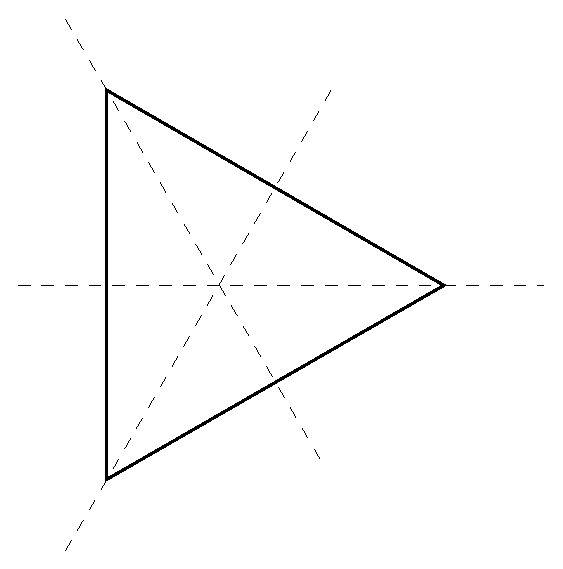
\includegraphics{D3triangle.or.eps}}

\Huge

%\psframe*[linecolor=white](-6.5,6)(-5.5,7)
%\psframe*[linecolor=white](6,-6.5)(7.2,-5.5)

\rput(5,0){$I_1$} \rput(-4,4.5){$I_2$} \rput(-4,-5){$I_3$}

\rput(3.2,0.5){A} \rput(-2.7,3.7){B} \rput(-3.7,-3.7){C}


% Use grid command below to place objects at specified coordinates.
% \psgrid[subgriddiv=1,griddots=10](-8,-8)(7,7)
}
\end{document}
